\documentclass[11pt]{amsart}
\usepackage[margin=1.2in]{geometry}
\usepackage{adjustbox}
\usepackage{amsmath,amssymb,amsthm,mathtools,booktabs,graphicx,microtype}
\usepackage[colorlinks=true,linkcolor=blue,citecolor=blue,urlcolor=blue]{hyperref}
\hypersetup{pdftitle={Gaussian Choice from Sparse Pairwise Interventions},pdfauthor={Bernd Johannes Wuebben},pdfsubject={Identification and estimation of Gaussian random utility models}}
\setlength{\emergencystretch}{2em}
\newtheorem{theorem}{Theorem}[section]
\newtheorem{proposition}[theorem]{Proposition}
\newtheorem{corollary}[theorem]{Corollary}
\theoremstyle{definition}\newtheorem{example}[theorem]{Example}
\theoremstyle{remark}\newtheorem{remark}[theorem]{Remark}
\newcommand{\R}{\mathbb R}\newcommand{\E}{\mathbb E}\newcommand{\Prob}{\mathbb P}
\newcommand{\one}{\mathbf 1}\newcommand{\diag}{\operatorname{diag}}
\newcommand{\rank}{\operatorname{rank}}\newcommand{\TV}{\operatorname{TV}}
\newcommand{\KL}{\operatorname{KL}}\newcommand{\argmax}{\operatorname*{arg\,max}}
\newcommand{\norm}[1]{\left\lVert#1\right\rVert}
\DeclareMathOperator{\tr}{tr}
\title[Gaussian Choice from Pairwise Interventions]{Gaussian Choice from Sparse Pairwise Interventions}
\author{Bernd Johannes Wuebben}
\subjclass[2020]{62H25 (primary); 62J12, 62K05 (secondary)}
\keywords{Random utility, multinomial probit, paired comparisons, factor analysis, experimental design, Euclidean distance reconstruction}
\date{September 5, 2026}
\begin{document}
\begin{abstract}
We study when binary choice experiments determine choice probabilities on larger menus under a stable Gaussian random utility model. The covariance is a rank-$r$ factor component plus an unknown nonnegative diagonal. Two calibrated additive treatment levels on each of a specified set of pairs identify the centered mean and covariance from $kn-k(k+1)/2$ pairs, where $k=3(r+1)$. The design uses three disjoint groups of $r+1$ alternatives whose factor loadings are affinely independent. Rectangular differences of pairwise contrast variances cancel the unknown diagonal, and three cross-group matrices determine the factor geometry. A constructive proof gives $O(nr^2+r^3)$ arithmetic and $O(nr)$ storage. Under bounded parameters, response overlap, and uniformly conditioned anchor groups, the inverse is locally stable with constants independent of $n$; repeated binary observations then yield a maximum-norm sampling bound and consistency for each fixed menu. Synthetic experiments examine finite-sample likelihood fitting, treatment placement, conditioning, and violations of the model. Menu-dependent means or covariance can preserve every pairwise response while changing larger-menu choice substantially. The random-pair recovery problem with unknown diagonal variance remains open.
\end{abstract}
\maketitle

\section{Introduction}
A binary experiment can be inexpensive to administer even when the eventual decision involves many alternatives. It is therefore useful to know whether experiments on selected pairs can determine substitution patterns on larger menus. Correlation is central to this question. Two alternatives with similar latent shocks can substitute strongly for one another, and their joint presence can change the probability of selecting a third alternative. A model fitted only to average pairwise preferences need not recover these effects.

This paper considers calibrated alternative-specific attribute interventions in a Gaussian random utility model. The attribute has a common additive effect on deterministic utility, and its manipulation leaves all other utilities and the joint shock law unchanged. A monetary bonus attached to choosing one alternative has this interpretation under quasi-linear utility with a common money coefficient. A numerical offset applied directly to a stochastic selection score gives an algorithmic interpretation. With a known coefficient, the intervention is measured in utility units; an unknown common nonzero coefficient leaves only a global utility scale unidentified. Observing the binary response at two levels determines both the mean difference and the variance of the utility contrast in that scale. If every pair is observed, double centering recovers the covariance on the space of contrasts. The main question is how to reduce the number of distinct experimental pairs when the covariance has a factor structure and the idiosyncratic variances are unknown.

Our main result gives a deterministic design with a number of pairs proportional to $nr$. Select three disjoint groups of $r+1$ alternatives and observe every pair containing at least one selected alternative. Each group must span the $r$-dimensional factor space affinely. Theorem~\ref{thm:anchors} identifies the idiosyncratic variances and the centered factor Gram matrix, uniquely within models of factor dimension at most $r$. This determines the full Gaussian contrast law and hence every menu and ranking probability under the maintained model.

The proof uses three pieces of information that a sparse graph need not otherwise provide. First, rectangular differences across disjoint groups remove the idiosyncratic variances as well as the squared loading norms. Second, the resulting three cross-Gram matrices determine the metric within one group. Third, distances to that group determine every remaining loading; residual variance sums on a triangle and a star then determine the diagonal component. Theorem~\ref{thm:stability} shows why the same formulas are stable near a well-conditioned configuration. Each recovered alternative depends on a fixed anchor block and its own measurements against that block. The resulting maximum-norm constants can therefore be chosen independently of the total number of alternatives.

The component ideas have established precedents. Location and scale restrictions in multinomial probit are treated by Bunch~\cite{bunch1991}. Unrestricted Thurstonian paired-comparison models have their own identification and estimation theory; Maydeu-Olivares and Hern\'andez~\cite{maydeu2007} use richer information that includes bivariate response margins. Here the observations are marginal binary responses under calibrated interventions. The distance-to-Gram identity is classical multidimensional scaling \cite{gower1966}. Most closely, Anderson and Rubin~\cite[Theorem~5.1]{anderson1956} identify factor structure from off-diagonal covariance information using disjoint full-rank blocks. Our reconstruction applies that principle to variance distances: rectangular differences first remove unknown diagonal noise, and an explicit experimental graph supplies the required blocks. The contribution is this observation design, its constructive recovery statement, and the associated local sampling analysis, rather than a new principle of factor rotation or probit normalization.

Randomly observed Euclidean distances provide a different route in the pure-factor case. Under their coherence hypotheses, Tasissa and Lai~\cite{tasissa2019} prove exact recovery by a centered positive-semidefinite matrix-completion program. Unknown idiosyncratic variances change the observation model, and that theorem does not directly supply the result proved here. We retain the distinction between designed observations, random-distance completion, and the behavior of a particular nonconvex numerical fit.

The experiments are entirely synthetic. They include exact reconstruction, a finite-sample comparison with independent Gaussian and logit models, and held-out menus whose outcomes are never used in fitting. They also examine seven violations of the assumptions. Separate appendices discuss a quadrature-based linear algebra reduction and a constrained probability allocation. These are consequences of established random utility geometry, included to clarify what additional computations become available after the contrast law is identified.

\section{What binary interventions identify}\label{sec:population}
There are $n$ alternatives with utilities
\begin{equation}\label{eq:model}
 U_i=\mu_i+\varepsilon_i,\qquad \varepsilon\sim N(0,\Sigma),\quad \Sigma\succeq0.
\end{equation}
For a nonempty menu $S\subseteq\{1,\ldots,n\}$, the choice is the maximizer of $U_i$ over $i\in S$. The vector $\mu$ and the joint shock law are the same for every menu. This is the menu-stability assumption. An experiment on the ordered pair $(i,j)$ adds $t$ to $U_i$ and leaves all other utilities and the shock distribution unchanged. Thus
\begin{equation}\label{eq:response}
 q_{ij}(t)=\Prob(U_i+t>U_j)
 =\Phi\left(\frac{\delta_{ij}+t}{s_{ij}}\right),\qquad
 \delta_{ij}=\mu_i-\mu_j,\quad s_{ij}^2=\Sigma_{ii}+\Sigma_{jj}-2\Sigma_{ij}.
\end{equation}
Here $\Phi$ is the standard normal cdf. We assume $s_{ij}>0$ on the pairs under discussion. Positive contrast variances on every pair ensure that ties have probability zero, even when $\Sigma$ is singular. Reversing a stored pair changes the sign convention for its mean difference and treatment.

Write $D_{ij}=s_{ij}^2$ for $i\ne j$, and set $D_{ii}=0$. Let
\[
 P=I-\frac{\one\one^T}{n},\qquad \bar\mu=P\mu,\qquad C=P\Sigma P.
\]
Here $C$ is the covariance of the centered utility shocks. For matrices, $\norm{\cdot}_{\max}$ denotes the largest absolute entry, and $\norm{\cdot}_F$ the Frobenius norm.

\begin{proposition}[Population inversion]\label{prop:population}
For $t_1<t_2$, two exact probabilities $q_{ij}(t_1),q_{ij}(t_2)$ identify $\delta_{ij}$ and $D_{ij}$. If all pairs are observed, they identify $\bar\mu$ and $C$, and hence the choice and ranking laws on all menus. Explicitly, with $z_\ell=\Phi^{-1}(q_{ij}(t_\ell))$,
\begin{equation}\label{eq:inverse}
 s_{ij}=\frac{t_2-t_1}{z_2-z_1},\qquad
 \delta_{ij}=s_{ij}z_1-t_1,\qquad C=-\tfrac12 PDP.
\end{equation}
Mean differences alone identify $\bar\mu$ whenever the observed graph is connected.
\end{proposition}
\begin{proof}
Equation~\eqref{eq:response} gives $z_\ell=(\delta_{ij}+t_\ell)/s_{ij}$, proving the first two formulas. If $a_i=\Sigma_{ii}$, then $D=a\one^T+\one a^T-2\Sigma$. Multiplication by $P$ on both sides gives the last formula. Connected edge differences recover $\mu$ up to a common constant. The Gaussian vector $PU$ has mean $\bar\mu$ and covariance $C$ and determines every utility ordering, proving the claim about menus and rankings.
\end{proof}

The identified covariance is a contrast covariance, not a distinguished covariance of utility levels. For symmetric $\Delta$, the equality $P\Delta P=0$ holds precisely when $\Delta=\one a^T+a\one^T$ for some $a\in\R^n$. To see this, decompose $\R^n$ into the span of $\one$ and its orthogonal complement: only the block acting within the complement must vanish. Both covariance representatives must of course be positive semidefinite. The observational freedom is larger than adding an independent common shock of variance $c$, which would only add $c\one\one^T$.

Calibration concerns the effect of an observable attribute, rather than direct observation of cardinal utility. To make this interpretation explicit, write $U_i=a_i+\beta x_i+\varepsilon_i$ and absorb the baseline attribute into $\mu_i=a_i+\beta x_i$. Changing only $x_i$ to $x_i+h$ gives
\begin{equation}\label{eq:attribute_response}
 q^x_{ij}(h)=\Phi\left(\frac{\delta_{ij}+\beta h}{s_{ij}}\right).
\end{equation}
For known nonzero $\beta$, the preceding formulas apply with $t=\beta h$. If $\beta$ is unknown but common to all experimental pairs, the probit slope has sign $\beta$ and magnitude $|\beta|/s_{ij}$. Writing the fitted probit line as $a_{ij}+b_{ij}h$, one recovers $\delta_{ij}/|\beta|=a_{ij}/|b_{ij}|$ and $D_{ij}/\beta^2=b_{ij}^{-2}$. The centered mean and covariance are therefore identified as $\bar\mu/|\beta|$ and $C/\beta^2$. This positive rescaling still determines untreated choices and rankings. It does not separately identify the attribute coefficient or covariance in an external cardinal utility scale.

A common coefficient is a restriction across the experiment, not merely within a pair. Unrestricted unknown pair-specific coefficients provide no common scale without additional restrictions. Unknown alternative-specific coefficients may impose cross-pair restrictions, but their identification is not covered here. Likewise, pooling respondents with different money coefficients or baseline preferences need not preserve a single Gaussian response model. Repeated observations must refer to the same maintained population law. Two treatment levels refer to two population probabilities; they do not mean that two binary observations suffice for estimation.

\begin{example}[A connected graph does not identify covariance]\label{ex:path}
Take $n=3$, $\mu=0$, and $\Sigma=vv^T+\tfrac12 I$. The loading vectors $v=(0,1,3)^T$ and $\widetilde v=(0,1,-1)^T$ yield
\[
 D=\begin{pmatrix}0&2&10\\2&0&5\\10&5&0\end{pmatrix},\qquad
 \widetilde D=\begin{pmatrix}0&2&2\\2&0&5\\2&5&0\end{pmatrix}.
\]
Every intervention response on edges $12$ and $23$ agrees. The probabilities of winning the three-alternative menu are approximately
\[
 (0.393060,0.171343,0.435597),\qquad (0.209785,0.395108,0.395108),
\]
respectively. These values can be obtained from centered bivariate Gaussian orthant probabilities: the probability that alternative $i$ wins is $1/4+(2\pi)^{-1}\arcsin(\rho_i)$, where
\[
 \rho_i=\frac{D_{ij}+D_{ik}-D_{jk}}{2\sqrt{D_{ij}D_{ik}}}.
\]
The connected path identifies mean differences but leaves a factor-distance ambiguity.
\end{example}

\section{A sparse design with unknown diagonal variances}\label{sec:anchors}
Assume now that
\begin{equation}\label{eq:factor}
 \Sigma=VV^T+\diag(d),\qquad V\in\R^{n\times r},\quad d_i\geq0.
\end{equation}
Let $v_i$ be row $i$ of $V$. For distinct alternatives,
\begin{equation}\label{eq:distance}
 D_{ij}=\norm{v_i-v_j}^2+d_i+d_j.
\end{equation}
The diagonal convention remains $D_{ii}=0$; formula~\eqref{eq:distance} is used only when $i\ne j$. Translating all loadings by the same vector and rotating their coordinates preserve the factor distances and the centered Gram matrix $PVV^TP$.

Choose three disjoint ordered groups
\[
 A=(a_0,\ldots,a_r),\quad B=(b_0,\ldots,b_r),\quad H=(h_0,\ldots,h_r).
\]
We call their members anchors, meaning simply the alternatives compared with every other alternative. The letter $H$ distinguishes the third group from the covariance $C$. Define the square matrices
\begin{equation}\label{eq:bases}
 X_{k\cdot}=v_{a_k}-v_{a_0},\quad
 Y_{k\cdot}=v_{b_k}-v_{b_0},\quad
 Z_{k\cdot}=v_{h_k}-v_{h_0},\qquad 1\leq k\leq r.
\end{equation}
A group is affinely independent precisely when its corresponding matrix is nonsingular.

\begin{theorem}[Three-group reconstruction]\label{thm:anchors}
Let $r\geq1$ and $n\geq3(r+1)$. Suppose~\eqref{eq:model} and~\eqref{eq:factor} hold, every pair has positive contrast variance, and $X,Y,Z$ in~\eqref{eq:bases} are nonsingular. Observe two calibrated treatment probabilities on each unordered pair having at least one endpoint in $A\cup B\cup H$. Then the observations uniquely determine
\[
 d,\qquad PVV^TP,\qquad \bar\mu,
\]
within the class of models of factor dimension at most $r$. In particular, they determine $C$ and every menu and ranking law. With $k=3(r+1)$, the design uses
\begin{equation}\label{eq:count}
 m=kn-\frac{k(k+1)}2
\end{equation}
distinct pairs. Reconstruction takes $O(nr^2+r^3)$ arithmetic operations and $O(nr)$ working storage when the covariance is returned in factor form.
\end{theorem}

\begin{proof}
Proposition~\ref{prop:population} recovers $D_{ij}$ and $\delta_{ij}$ on every observed pair. We give a reconstruction from these values.

\emph{Recover a factor metric from three cross-group matrices.}
For $1\leq k,l\leq r$, form
\begin{equation}\label{eq:cross}
 (K_{AB})_{kl}=-\tfrac12
 (D_{a_kb_l}-D_{a_kb_0}-D_{a_0b_l}+D_{a_0b_0}).
\end{equation}
Each distance compares an alternative in $A$ with one in $B$, so no diagonal entry of $D$ occurs. Substituting~\eqref{eq:distance} cancels every $d_i$ and every squared loading norm, leaving
\[
 K_{AB}=XY^T.
\]
The same construction gives $K_{AH}=XZ^T$ and $K_{BH}=YZ^T$. Since the bases are nonsingular,
\begin{equation}\label{eq:metric}
 G_A=K_{AB}K_{BH}^{-T}K_{AH}^T=XX^T.
\end{equation}
Let $X_*$ be the lower triangular Cholesky factor of $G_A$. There is an orthogonal matrix $Q$ with $X_*=XQ$.

\emph{Recover coordinates relative to $b_0$.}
For $i\notin A$, define the row vector
\begin{equation}\label{eq:outside}
 (u_i)_k=-\tfrac12
 (D_{ia_k}-D_{ia_0}-D_{b_0a_k}+D_{b_0a_0}),\qquad
 w_i=u_iX_*^{-T}.
\end{equation}
All required pairs are observed and join distinct alternatives. Direct expansion gives $u_i=(v_i-v_{b_0})X^T$, and therefore $w_i=(v_i-v_{b_0})Q$. In particular, $w_{b_0}=0$, the entire group $B$ is recovered, and $w_{h_0}$ is known. Set $(Y_*)_{l\cdot}=w_{b_l}-w_{b_0}= (YQ)_{l\cdot}$. For $i\in A$, form
\begin{equation}\label{eq:inside}
 (z_i)_l=-\tfrac12
 (D_{ib_l}-D_{ib_0}-D_{h_0b_l}+D_{h_0b_0}),\qquad
 w_i=w_{h_0}+z_iY_*^{-T}.
\end{equation}
The same expansion gives $w_i=(v_i-v_{b_0})Q$. Thus all squared factor distances and $PWW^TP=PVV^TP$ have been recovered.

\emph{Recover the diagonal and the means.}
For observed edges let $R_{ij}=D_{ij}-\norm{w_i-w_j}^2=d_i+d_j$. A triangle of anchors gives
\begin{equation}\label{eq:diagonal}
 d_{a_0}=\tfrac12(R_{a_0b_0}+R_{a_0h_0}-R_{b_0h_0}),\qquad
 d_i=R_{ia_0}-d_{a_0}\quad(i\ne a_0).
\end{equation}
Every edge in this star is observed. Likewise set $\nu_{a_0}=0$, $\nu_i=\delta_{ia_0}$ and recover $\bar\mu=P\nu$. Finally
\[
 C=PWW^TP+P\diag(d)P.
\]

\emph{Uniqueness and cost.}
In any other representation with at most $r$ factors, $K_{AB}$ has rank $r$, so the factor dimension is $r$ and all three cross-group bases are nonsingular. Equations~\eqref{eq:metric}--\eqref{eq:diagonal} then recover the same loading configuration up to Euclidean motion and the same $d$. This proves uniqueness in the asserted model class. There are $k(n-k)+k(k-1)/2$ observed pairs, giving~\eqref{eq:count}. The anchor matrices require $O(r^3)$ work; a fixed number of matrix-vector operations of size $r$ for each alternative require $O(nr^2)$ work. Storing the observed pairs, recovered loadings, means and diagonal requires $O(nr)$ space. Materializing a dense covariance would instead require $O(n^2)$ storage.
\end{proof}

The proof adapts the off-diagonal factor-identification mechanism of Anderson and Rubin~\cite{anderson1956} to the distance measurements supplied by interventions. Its rank restriction is substantive: it does not exclude an arbitrary higher-rank covariance agreeing with the observed distances. The theorem also assumes a design whose anchor groups satisfy the rank condition. If all loading entries have a joint distribution absolutely continuous with respect to Lebesgue measure, any fixed three disjoint groups are affinely independent with probability one. This follows because each determinant is a nonzero polynomial. Almost-sure invertibility supplies no uniform bound on the inverses.

\begin{example}[One factor]
When $r=1$, choose two alternatives in each of three groups. If their loading differences are the nonzero scalars $x,y,z$, the three rectangular differences are $xy,xz,yz$. Their combination $(xy)(xz)/(yz)=x^2$ determines the squared scale of the first difference. Distances to its two endpoints then locate every other loading on the line, up to a common reflection and translation. The residual triangle separates the idiosyncratic variances. Six anchors use $6n-21$ pairs. The graph contains information absent from the three-vertex path in Example~\ref{ex:path}.
\end{example}

\subsection{Relation to random distance completion}
If $d=0$, let $B=PVV^TP$. An observed distance is the linear functional
\[
 D_{ij}=\langle B,(e_i-e_j)(e_i-e_j)^T\rangle.
\]
The centered positive-semidefinite completion problem minimizes $\tr(B)$ subject to these equalities, $B\succeq0$ and $B\one=0$. Under the three coherence conditions in equations (12)--(14) of Tasissa and Lai~\cite{tasissa2019}, their Theorem~1 gives a sufficient number of uniformly sampled measurements, with replacement, of order $nr\nu\log^2 n$ for fixed probability exponent and coherence parameter $\nu$ bounded below by a positive constant. That conclusion concerns their convex program and their hypotheses. More recently, Ghosh, Tasissa and K\"ummerle~\cite{ghosh2024} analyze an iteratively reweighted least-squares algorithm with a local quadratic convergence guarantee from a sufficiently close initialization under incoherence and random sampling. Neither theorem applies directly to our stress optimizer.

In~\eqref{eq:distance}, unknown $d_i+d_j$ adds a structured nuisance component. Double centering a complete $D$ still works, but a partial distance matrix cannot be filled with zeros before centering. Theorem~\ref{thm:anchors} supplies a designed solution with unknown $d$. A comparable random-pair theorem in that model would require additional analysis of uniqueness, conditioning and an estimator. The random-graph experiments below concern the pure-factor model and a stress minimizer; they do not implement the cited convex program.

\section{Local stability and repeated observations}\label{sec:stability}
The exact inverse can amplify small errors when an anchor group is nearly affinely dependent. We first state a uniform local result on a restricted parameter class. This also specifies the scope of the sampling guarantee.

Fix $r$, positive constants $M,\kappa,d_*,\tau$, and $0<\rho<1/2$. Translate the loadings so that $v_{b_0}=0$ and the means so that $\mu_{a_0}=0$. Assume
\begin{equation}\label{eq:compact}
 \norm{v_i}\leq M,\quad |\mu_i|\leq M,\quad d_*\leq d_i\leq M,
 \quad \sigma_{\min}(X),\sigma_{\min}(Y),\sigma_{\min}(Z)\geq\kappa.
\end{equation}
For each observed pair the two treatments may differ from those used on other pairs, but satisfy
\begin{equation}\label{eq:overlap}
 |t_\ell|\leq M,\qquad t_2-t_1\geq\tau,\qquad
 \rho\leq q_{ij}(t_\ell)\leq1-\rho.
\end{equation}
The constants below may depend on these fixed quantities, but not on $n$.

Define a local estimator as follows. Apply~\eqref{eq:inverse} to the estimated responses. Use~\eqref{eq:metric}, replace its estimated right side by its symmetric part, and take its Cholesky factor if positive definite. Apply~\eqref{eq:outside}--\eqref{eq:diagonal} and the mean star. Center the recovered coordinates and means. If an inverse does not exist, the Cholesky factor does not exist, a recovered $d_i$ is nonpositive, or an inferred pair scale is nonpositive, flag the estimate as invalid. A fixed valid default model can be returned on this event. Thus the estimator is defined on all samples; the theorem describes a neighborhood where no flag occurs.

\begin{theorem}[Uniform local stability]\label{thm:stability}
Under~\eqref{eq:compact}--\eqref{eq:overlap}, there exist $\epsilon_0>0$ and $K<\infty$, independent of $n$, such that if
\[
 \max_{(i,j),\ell}|\widehat q_{ij}(t_\ell)-q_{ij}(t_\ell)|\leq\epsilon\leq\epsilon_0,
\]
the local estimator is valid and satisfies
\begin{equation}\label{eq:stable}
 \norm{\widehat{\bar\mu}-\bar\mu}_\infty
 +\norm{\widehat d-d}_\infty
 +\norm{\widehat D-D}_{\max}
 +\norm{\widehat C-C}_{\max}\leq K\epsilon.
\end{equation}
Here $\widehat D$ denotes all distances implied by the recovered factor model, with zero diagonal, including unobserved pairs.
\end{theorem}
\begin{proof}
The inverse normal cdf has bounded derivative on $[\rho/2,1-\rho/2]$. By~\eqref{eq:compact}, every true scale is at most $\sqrt{4M^2+2M}$. Thus the true denominator $z_2-z_1=(t_2-t_1)/s_{ij}$ is at least $\tau/\sqrt{4M^2+2M}$. Equations~\eqref{eq:inverse} therefore have bounded derivatives on a common neighborhood of the admissible pair data. They recover every observed $D_{ij}$ and $\delta_{ij}$ with error at most $K_1\epsilon$.

Each entry of a cross-group matrix is a fixed linear combination of four distances. The smallest singular value of $K_{BH}=YZ^T$ is at least $\kappa^2$, while that of $G_A=XX^T$ is at least $\kappa^2$. The true anchor data belong to a compact set of fixed dimension, independent of $n$. Matrix inversion, symmetrization and Cholesky factorization are continuously differentiable on a common neighborhood of this set. Consequently the reconstructed $X_*$ differs by at most $K_2\epsilon$ from the Cholesky factor for the true configuration and remains nonsingular.

For each alternative outside $A$, formula~\eqref{eq:outside} depends only on this anchor block and a vector of $r+1$ distances involving that alternative, together with the fixed reference distances. These inputs are uniformly bounded. Its derivative is therefore uniformly bounded independently of which alternative is used. The recovered group $B$ remains a nonsingular basis, and the same reasoning applies to~\eqref{eq:inside}. We obtain
\[
 \max_i\norm{\widehat w_i-w_i}\leq K_3\epsilon
\]
in the respective Cholesky coordinate systems; the true $w_i$ are bounded by $M$. The residual formulas~\eqref{eq:diagonal} then give maximum error at most $K_4\epsilon$ in $d$. Reducing $\epsilon_0$ if necessary keeps all recovered variances above $d_*/2$.

For arbitrary $i,j$, the difference between the reconstructed and true squared loading distances is bounded by a constant times the maximum coordinate error, since both configurations are bounded. Adding the two diagonal errors proves the bound for all entries of $D$. The mean star has error at most $K_1\epsilon$ before centering and at most $2K_1\epsilon$ afterwards. Finally, for any matrix $E$, $\norm{PEP}_{\max}\leq4\norm E_{\max}$. Applying $C=-PDP/2$ proves the covariance bound. All neighborhoods and constants used for target alternatives depend on fixed-dimensional bounded input sets, so the number of alternatives does not enter them.
\end{proof}

\begin{corollary}[A maximum-norm sampling bound]\label{cor:sampling}
At each of the two fixed treatment levels on each of the $m$ observed pairs, collect $N$ independent Bernoulli observations with the specified response probability. Under~\eqref{eq:compact}--\eqref{eq:overlap}, there are constants $K_0,K_1$ independent of $n$ such that, for $0<\alpha<1$ and $N\geq K_0\log(4m/\alpha)$, the local estimator satisfies the bound in~\eqref{eq:stable} with right side
\begin{equation}\label{eq:rate}
 K_1\sqrt{\frac{\log(4m/\alpha)}{N}}
\end{equation}
with probability at least $1-\alpha$. The total number of binary observations is $2mN$.
\end{corollary}
\begin{proof}
Let $\widehat q$ be each cell's empirical frequency, clipped to $[\rho/2,1-\rho/2]$. Clipping cannot increase its distance to the true $q$. Hoeffding's inequality and a union bound over $2m$ cells give
\[
 \Prob\left(\max|\widehat q-q|>u\right)\leq4m e^{-2Nu^2}.
\]
Take $u=\sqrt{\log(4m/\alpha)/(2N)}$ and choose $K_0$ so that $u\leq\epsilon_0$. Apply Theorem~\ref{thm:stability}. Independence across distinct cells is unnecessary for this union bound; the within-cell binomial assumption suffices.
\end{proof}

The bound controls entries, not relative Frobenius error uniformly over all possible covariances. Its constants depend on anchor conditioning and overlap. It applies to the local algebraic estimator and fixed treatments. The constrained pair fits, adaptive treatments and nonconvex likelihood refinement used in the experiments are separate procedures.

\begin{proposition}[From parameter error to menu error]\label{prop:menu}
Suppose $d_i\geq d_*>0$ in the true model. Let a fitted Gaussian model have centered mean and covariance errors bounded entrywise by $\epsilon_\mu$ and $\epsilon_C$, respectively. On a menu of size $s\geq2$, put $p=s-1$. If $4p\epsilon_C/d_*\leq1/2$, the total variation distance between the true and fitted choice laws, and also between their full ranking laws, is at most
\begin{equation}\label{eq:tv}
 \sqrt{\frac{p\epsilon_\mu^2}{d_*}
       +\frac{4p^2\epsilon_C^2}{d_*^2}}.
\end{equation}
\end{proposition}
\begin{proof}
Choose one alternative as a base and let $T$ be the $p$ by $n$ matrix whose rows subtract its coordinate from each other menu coordinate. The true contrast law is $N(a,\Omega)$ with $a=T\bar\mu$ and $\Omega=TCT^T=T\Sigma T^T$. Since $T\diag(d)T^T\succeq d_*TT^T$ and $TT^T=I_p+\one\one^T$, we have $\Omega\succeq d_*I_p$. The fitted mean error has Euclidean norm at most $2\sqrt p\epsilon_\mu$, and every fitted covariance error entry is at most $4\epsilon_C$, so its Frobenius norm is at most $4p\epsilon_C$.

Set $E=\Omega^{-1/2}(\widehat\Omega-\Omega)\Omega^{-1/2}$. Its operator norm is at most $1/2$. If $\lambda_j$ are its eigenvalues, then $\lambda_j-\log(1+\lambda_j)\leq\lambda_j^2$ for $|\lambda_j|\leq1/2$. The Gaussian relative entropy formula yields
\[
 \KL\bigl(N(\widehat a,\widehat\Omega)\,\Vert\,N(a,\Omega)\bigr)
 \leq\frac12\left(\frac{4p\epsilon_\mu^2}{d_*}
                  +\frac{16p^2\epsilon_C^2}{d_*^2}\right).
\]
Pinsker's inequality gives~\eqref{eq:tv}. Both the winner and the entire ranking are measurable functions of the contrast vector, so total variation cannot increase when passing to either outcome.
\end{proof}

For each fixed menu, Corollary~\ref{cor:sampling} and Proposition~\ref{prop:menu} imply consistency as $\log(m)/N\to0$ within the stated uniformly conditioned class. The explicit dependence on $s$ prevents interpreting this as a dimension-free guarantee for arbitrarily large menus.

\section{Estimation and treatment placement}\label{sec:estimation}
For an observed pair, write $q(t)=\Phi(a+bt)$ with $a=\delta/s$ and $b=1/s>0$. If $y_\ell$ successes occur in $N_\ell$ trials at $t_\ell$, we maximize the binomial log likelihood
\begin{equation}\label{eq:pairlik}
 \ell(a,b)=\sum_\ell\{y_\ell\log\Phi(a+bt_\ell)
 +(N_\ell-y_\ell)\log\Phi(-a-bt_\ell)\}.
\end{equation}
The experiments constrain $a\in[-12,12]$ and $b\in[0.05,10]$. These bounds prevent infinite estimates under separation and impose explicit restrictions on inferred scales. The estimates are $\widehat\delta=\widehat a/\widehat b$ and $\widehat D=\widehat b^{-2}$.

Writing $\phi$ for the standard normal density, the expected information for $(a,b)$ from one observation at $t$ is
\begin{equation}\label{eq:information}
 I(t)=\frac{\phi(a+bt)^2}{\Phi(a+bt)\Phi(-a-bt)}
 \begin{pmatrix}1&t\\t&t^2\end{pmatrix}.
\end{equation}
For equal allocation at standardized predictors $\pm c$, its determinant is proportional to
\[
 c^2\left\{\frac{\phi(c)^2}{\Phi(c)\Phi(-c)}\right\}^2.
\]
The familiar probit design value is $c\simeq1.13810128$, corresponding to probabilities about $0.128$ and $0.872$. Locally optimal sensitivity-test designs and sequential approximations to them are classical; see Neyer~\cite{neyer1994}. This calculation provides treatment placement when the pair parameters are approximately known, rather than a new optimal-design result.

We compare three designs with $2N$ observations per pair. The fixed design uses $t=\pm1.5$. The adaptive design first uses $N_0=\max(10,\lfloor0.2N\rfloor)$ trials at each fixed level, estimates the pair parameters, and places the remaining $N-N_0$ trials at each of
\[
 t_\pm=\operatorname{clip}_{[-8,8]}
 \bigl(-\widehat\delta_{\rm pilot}\pm1.13810128\sqrt{\widehat D_{\rm pilot}}\bigr).
\]
All four cells enter the final likelihood. The oracle design uses the true pair parameters to place its two levels. It is an information benchmark unavailable to an experimenter. The adaptive decisions use only pilot data; no multiway outcomes or true parameters enter them.

Let $E$ be the set of observed pairs. After fitting pairs, unweighted graph least squares estimates centered means. To estimate factor structure, we minimize weighted observed-distance stress,
\begin{equation}\label{eq:stress}
 \sum_{(i,j)\in E}w_{ij}
 \bigl(\norm{x_i-x_j}^2+e_i+e_j-\widehat D_{ij}\bigr)^2,
 \qquad e_i\geq0.
\end{equation}
The weights are reciprocal delta-method variance estimates from~\eqref{eq:information}, clipped to $[0.01,1000]$ after flooring the estimated variance at $10^{-6}$. We use both an overdetermined version of the anchor construction and a spectral initialization, and select the fitted stress solution by its observed objective. For the anchor initialization, each group has eight alternatives when $r=3$. Cross-matrix inverses are replaced by rank-$r$ pseudoinverses, and the symmetrized recovered Gram matrix is truncated to its leading positive eigenspace. Negative diagonal estimates are projected to zero. This regularized initialization need not reconstruct noisy distances accurately.

Finally, a joint fit optimizes the binomial likelihood with
\[
 \eta_{ij\ell}=\frac{\mu_i-\mu_j+t_\ell}
 {\sqrt{\norm{v_i-v_j}^2+d_i+d_j}},\qquad d_i\geq0.02,
\]
starting from the selected stress solution. Centering fixes the mean and loading translation freedoms. We use a bounded quasi-Newton routine with analytic gradients. Numerical convergence of this nonconvex fit does not certify a global likelihood maximum. As baselines, an independent Gaussian model estimates one mean and one diagonal variance per alternative, and a logit model estimates item scores and one common positive treatment coefficient. Each baseline receives exactly the same pair outcomes and treatment levels as the correlated fit.

\section{Synthetic experiments}\label{sec:experiments}
All results below are generated from specified probability models. There are no respondent data or estimates of actual demand. Each parameter configuration has three seeds; this is a limited simulation grid, not a precise estimate of an average risk over a population of applications. Tables report means over the three seeds unless stated otherwise. Source files, seeds, software versions and per-case outputs accompany the manuscript.

\subsection{Population recovery, conditioning and scale}
The full-pair validation uses eight cases covering factor-plus-diagonal, unrestricted positive-definite and independent covariance, and checks the path counterexample in Example~\ref{ex:path}. Separate Gaussian orthant and Monte Carlo calculations compare the original and recovered choice laws. The anchor grid uses $n\in\{50,200,1000\}$, $r\in\{1,2,5,10\}$ and three seeds, with independent loadings $N(0,1/r)$ and $d_i$ uniform on $[0.3,1]$. All 36 reconstructions have small relative centered-covariance error (Table~\ref{tab:anchors}). These are numerical checks of the constructive formulas.
\begin{table}[htbp]\centering\small
\begin{tabular}{rrrr}
\toprule
$n$ & $r$ & Pairs & Maximum relative error \\
\midrule
50 & 1 & 279 & $4.1\times10^{-15}$ \\
50 & 2 & 405 & $9.7\times10^{-13}$ \\
50 & 5 & 729 & $9.1\times10^{-10}$ \\
50 & 10 & 1089 & $4.9\times10^{-13}$ \\
200 & 1 & 1179 & $1.3\times10^{-15}$ \\
200 & 2 & 1755 & $1.0\times10^{-12}$ \\
200 & 5 & 3429 & $1.3\times10^{-14}$ \\
200 & 10 & 6039 & $5.5\times10^{-14}$ \\
1000 & 1 & 5979 & $1.5\times10^{-14}$ \\
1000 & 2 & 8955 & $2.1\times10^{-13}$ \\
1000 & 5 & 17829 & $9.3\times10^{-13}$ \\
1000 & 10 & 32439 & $8.7\times10^{-14}$ \\
\bottomrule
\end{tabular}

\caption{Noiseless anchor reconstruction. The last column is the maximum of $\norm{\widehat C-C}_F/\norm C_F$ over three seeds. The pair count includes every pair involving the $3(r+1)$ anchors.}\label{tab:anchors}
\end{table}

A conditioning experiment fixes $n=100,r=2$ and multiplies the second loading coordinate of the nine anchors by a factor ranging from $1$ to $10^{-3}$. With the smallest factor, an observed-distance perturbation bounded by $10^{-6}$ produces approximately $0.043$ relative held-out distance error and five negative raw estimates of $d_i$. That output is an invalid covariance decomposition. It illustrates the role of the conditioning hypothesis; noiseless uniqueness alone does not protect the algebraic inverse from measurement noise.

A separate rank-three calculation evaluates two population responses on the minimal 12-anchor design and reconstructs up to one million alternatives (Table~\ref{tab:scaling}). It stores the observed edges and factor representation, and compares distances on 20,000 randomly sampled pairs. It does not form a dense covariance or evaluate a million-alternative choice probability. Times are single-run wall times on macOS with an ARM processor and a single numerical-library thread; they exclude experimental data collection and should be read as implementation measurements.
\begin{table}[htbp]\centering\small
\begin{tabular}{rrrrr}
\toprule
$n$ & Pairs & Response (s) & Inverse (s) & Distance error \\
\midrule
1,000 & 11,922 & 0.0008 & 0.0006 & $1.1\times10^{-14}$ \\
10,000 & 119,922 & 0.0072 & 0.0037 & $4.0\times10^{-15}$ \\
100,000 & 1,199,922 & 0.0674 & 0.0364 & $6.3\times10^{-15}$ \\
1,000,000 & 11,999,922 & 0.6657 & 0.3875 & $5.2\times10^{-15}$ \\
\bottomrule
\end{tabular}

\caption{Population response evaluation and anchor inversion, $r=3$. Distance error is relative Euclidean error over 20,000 sampled pair variances. Population probabilities, rather than finite binary samples, are supplied to the inverse.}\label{tab:scaling}
\end{table}

\subsection{Random pairs in the pure-factor model}
We also draw distinct random pairs without replacement, with
\[
 m=\min\{\lceil c nr\log n\rceil,n(n-1)/2\},\qquad d=0.
\]
The main grid has $n\in\{200,500,1000\}$, $r\in\{2,5,10\}$ and $c\in\{0.5,1,2,4,8\}$, with three seeds. Nine additional cases use $n=200,r=2$ and $c\in\{0.05,0.1,0.25\}$. A spectral initialization followed by unweighted stress minimization achieves relative centered-covariance error below $10^{-4}$ in 126 of 144 cases. Figure~\ref{fig:random} retains the failures. The smallest pair counts can leave structural ambiguities, while other failures may reflect the optimizer. This experiment does not separate those explanations and supplies no random-design identification theorem.
\begin{figure}[htbp]\centering
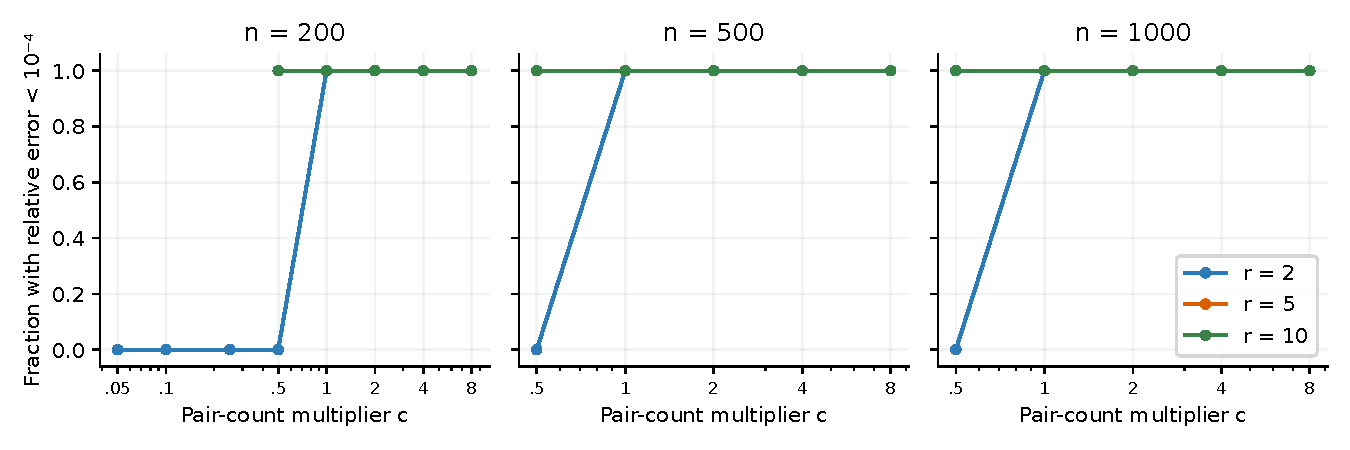
\includegraphics[width=\textwidth]{figures/random.pdf}
\caption{Pure-factor random-pair stress recovery. Each plotted fraction uses three seeds. Pair counts are capped at the complete graph; different $c$ values can therefore produce the same graph size. Success denotes numerical relative covariance error below $10^{-4}$. The $r=5$ and $r=10$ curves coincide on this grid.}\label{fig:random}
\end{figure}

\subsection{Finite samples and held-out menus}
The finite-sample model has $n=100,r=3$, independent $\mu_i\sim N(0,0.4^2)$, loading entries $N(0,0.8^2)$, and $d_i$ uniform on $[0.4,1]$. The anchor design uses 24 anchors in three groups of eight, hence 2,100 pairs. The complete design uses 4,950 pairs. We cross the two graphs with three treatment designs, five values $N\in\{50,100,250,500,1000\}$ and three seeds, giving 90 cases. At a given $N$, the complete graph uses more total binary observations; it is not a comparison at equal total budget.

For each case we evaluate a random five-alternative menu, a random 20-alternative menu, the full 100-alternative menu, and the 19-alternative menu obtained by deleting the largest-true-mean item from the 20-alternative menu. This last selection uses the simulation truth only to define the evaluation scenario. Model fitting uses no outcome on these menus. Independent simulations with 65,536 draws per model estimate their choice probabilities. A second simulation from the true model measures the Monte Carlo comparison floor, about $0.008$ mean total variation on the 20-alternative menus. The floor is a diagnostic, not a bias correction for individual entries.

\begin{table}[htbp]\centering\small
\begin{tabular}{lrrrrrrr}
\toprule
Design & $N$ & $C$ error & Two-stage & Joint & Indep. & Logit & Joint, 100 \\
\midrule
Anchors & 50 & 0.344 & 0.224 & 0.095 & 0.165 & 0.290 & 0.169 \\
Anchors & 250 & 0.137 & 0.040 & 0.035 & 0.140 & 0.293 & 0.077 \\
Anchors & 1000 & 0.070 & 0.020 & 0.021 & 0.134 & 0.292 & 0.042 \\
Complete & 50 & 0.188 & 0.124 & 0.054 & 0.103 & 0.288 & 0.103 \\
Complete & 250 & 0.072 & 0.021 & 0.019 & 0.106 & 0.290 & 0.039 \\
Complete & 1000 & 0.036 & 0.010 & 0.010 & 0.105 & 0.290 & 0.024 \\
\bottomrule
\end{tabular}

\caption{Adaptive treatment design, three-seed means. The covariance column is relative Frobenius error for the joint fit. The next four columns give 20-alternative total variation for the two-stage correlated, joint correlated, independent Gaussian and logit fits. The last column gives the joint fit's 100-alternative total variation.}\label{tab:finite}
\end{table}

The correlated fits improve as observations accumulate (Table~\ref{tab:finite}). Under adaptive treatment placement, mean joint covariance error on the anchor graph decreases from $0.344$ at $N=50$ to $0.070$ at $N=1000$, while mean 20-alternative total variation decreases from $0.095$ to $0.021$. The independent Gaussian and logit baselines retain larger menu errors in these correlated data-generating models. These results establish performance on this grid, with known factor dimension, rather than uniform dominance over other models or designs.

\begin{figure}[htbp]\centering
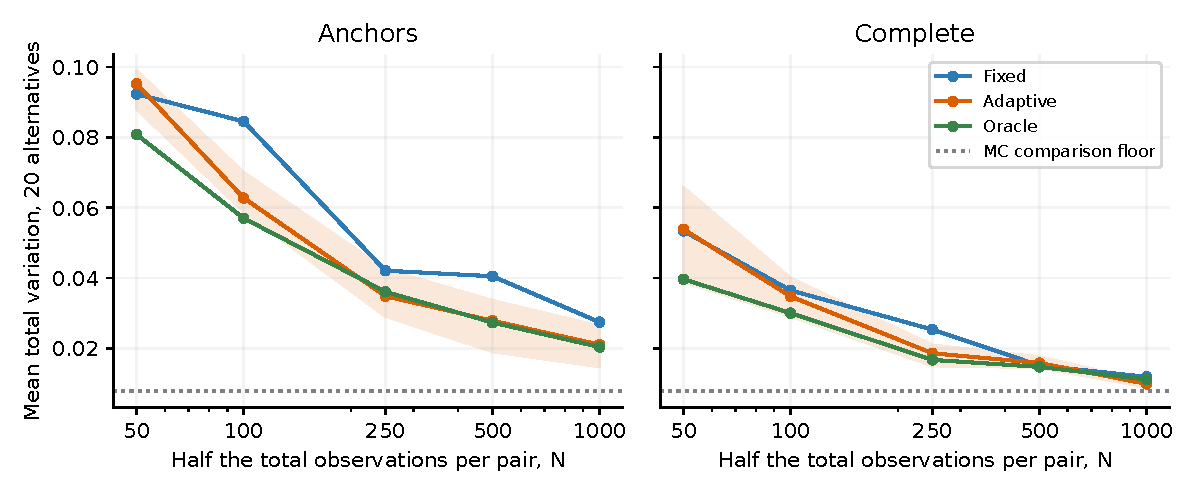
\includegraphics[width=.96\textwidth]{figures/finite.pdf}
\caption{Joint fit's 20-alternative error under fixed, adaptive and oracle treatment placement. Lines are three-seed means; shading gives the adaptive design's minimum and maximum across seeds. The oracle uses true parameters. Each graph has the same $2N$ trials per pair across treatment designs, but the complete graph uses more pairs.}\label{fig:finite}
\end{figure}

Figure~\ref{fig:finite} shows that adaptive treatment placement can help at larger sample sizes, but its pilot cost and estimation error can offset the gain at $N=50$. Joint likelihood refinement is particularly useful when the two-stage fit is poor. All 90 final joint fits report numerical convergence; implementation checks are described in Appendix~\ref{app:reproduce}.

For the deletion experiment, the diversion share to retained alternative $j$ is $(p_j^{\rm after}-p_j^{\rm before})/p_i^{\rm before}$, where $i$ is removed. Table~\ref{tab:diversion} reports the root mean squared error across retained alternatives. Monte Carlo noise affects both its numerator and denominator, and can be amplified for rarely chosen removed alternatives.
\begin{table}[htbp]\centering\small
\begin{tabular}{lrrrr}
\toprule
Design & $N$ & Joint & Indep. & Logit \\
\midrule
Anchors & 50 & 0.023 & 0.040 & 0.042 \\
Anchors & 250 & 0.009 & 0.039 & 0.042 \\
Anchors & 1000 & 0.005 & 0.039 & 0.042 \\
Complete & 50 & 0.011 & 0.038 & 0.042 \\
Complete & 250 & 0.006 & 0.037 & 0.042 \\
Complete & 1000 & 0.005 & 0.038 & 0.042 \\
\bottomrule
\end{tabular}

\caption{Deletion diversion-share RMSE under adaptive treatment placement, averaged across three seeds. No deletion outcome enters the fit.}\label{tab:diversion}
\end{table}

\subsection{Violations of the assumptions}\label{sec:misspec}
We use $n=30,r=2$ and all 435 pairs to separate model misspecification from sparse completion. Each scenario has three seeds. Except for the nonadditive case, the two training responses at $t=\pm1.5$ are calculated from population formulas. After pair inversion and mean least squares, we double center the complete distance matrix and project negative covariance eigenvalues to zero without imposing a factor-rank restriction. We then compare predictions with responses at $t=-0.75,0,0.75$ and choices on menus of sizes 5, 10, 20 and 30. Menu probabilities use 131,072 independent draws per model.

\begin{table}[htbp]\centering\small
\begin{tabular}{lrrr}
\toprule
Data-generating model & Pair RMSE & Menu TV & Range \\
\midrule
Gaussian control & 0.000 & 0.005 & 0.004--0.005 \\
Student $t_5$ & 0.016 & 0.045 & 0.036--0.052 \\
Gaussian mixture & 0.053 & 0.535 & 0.491--0.620 \\
Menu-dependent covariance & 0.000 & 0.139 & 0.074--0.207 \\
Context-dependent means & 0.000 & 0.201 & 0.184--0.233 \\
Treatment-dependent variance & 0.033 & 0.080 & 0.063--0.091 \\
Pair-specific treatment scale & 0.023 & 0.293 & 0.286--0.309 \\
Nonadditive utility & 0.068 & 0.129 & 0.082--0.188 \\
\bottomrule
\end{tabular}

\caption{Misspecification experiments. Pair RMSE uses three held-out treatment levels on every pair. Menu TV is total variation on a 20-alternative menu; the range is over three seeds. Entries printed as $0.000$ in the Gaussian, menu-covariance and context rows are below $10^{-12}$.}\label{tab:misspec}
\end{table}

The seven violations are specified in Appendix~\ref{app:misspec}. The largest discrepancies on this grid arise from a two-component Gaussian mixture and pair-specific treatment coefficients. More fundamentally, the menu-covariance and context scenarios leave all binary response curves exactly Gaussian with the training parameters, yet change the larger-menu law. Their held-out pair errors vanish while their average 20-alternative errors are $0.139$ and $0.201$. Even complete intervention curves on every pair cannot test unrestricted menu stability. Conversely, a discrepancy on held-out treatments or menus need not identify a unique violated assumption.

\section{Discussion}
A calibrated pairwise intervention reveals a variance distance as well as a mean difference. Three affinely independent anchor groups convert these distances into a complete factor-plus-diagonal contrast model using $O(nr)$ distinct pairs. The algebra is explicit, and its local stability follows from the fixed size of the anchor calculations. The statistical cost also depends on the repetitions needed to estimate the binary probabilities: $O(nr)$ pairs alone is not a finite-observation sample-complexity claim.

Treatment calibration and menu stability require substantive justification in an application. Controlled monetary bonuses require a common additive utility response over the experimental range, with no accompanying changes in perceived quality, other alternatives, or the shock law. Direct score offsets can enforce the additive intervention in an algorithmic selector if they are applied after score generation and the same score law governs both binary and larger-menu selection. Gaussianity and factor structure remain separate assumptions. Binary identification is useful when only comparison outcomes are accessible; when the full random score vectors are observed, their contrasts can be estimated directly. These settings motivate the intervention assumption without establishing an empirical application. The synthetic violations show why accurate pairwise fit cannot replace validation on deployment menus.

Several questions remain. One is whether randomly chosen pairs permit comparably efficient recovery with an unknown diagonal component. Another is how to select well-conditioned anchors from preliminary data when factor dimension and loading geometry are unknown. The present finite-sample procedures use the true factor dimension and numerical local optimization; neither rank selection nor global likelihood convergence is established here.

The Gaussian joint law is also essential to the conclusion as stated. A known elliptical family with a fixed radial generator may admit an analogous contrast reconstruction after replacing the probit inverse by its known standardized marginal inverse, provided that inverse is well defined; outside finite-moment families the recovered deterministic parameter is a location rather than a mean. Unrestricted dependence or a collection of Gaussian pairwise marginals does not by itself supply the joint contrast law. Extensions beyond a specified joint family therefore require additional observations or restrictions.

\appendix
\section{Quadrature and a reduced Laplacian solve}\label{app:quadrature}
This appendix records a computational consequence of established random utility derivative formulas. It is separate from the sparse identification argument. For independent Gaussian utilities with positive variances, write $f_i(x)$ and $F_i(x)$ for their densities and cdfs, including their deterministic means. Define the expected surplus by $S(\mu)=\E\max_i(\mu_i+\varepsilon_i)$, and set
\[
 G(x)=\prod_iF_i(x),\qquad a_i(x)=f_i(x)/F_i(x).
\]
The off-diagonal tie-density weight between alternatives $i$ and $j$ is
\begin{equation}\label{eq:tie}
 w_{ij}=\int_\R f_i(x)f_j(x)\prod_{k\ne i,j}F_k(x)\,dx
       =\int_\R G(x)a_i(x)a_j(x)\,dx\quad(i\ne j).
\end{equation}
Differentiating the continuum choice integral with respect to another mean gives $-w_{ij}$. Translation invariance gives the diagonal as the sum of the off-diagonal weights. Thus the surplus Hessian is a weighted graph Laplacian. Integral derivative formulas and scalable contest inversion are developed by Cotton~\cite{cotton2021,cotton2026}; the latter explicitly describes the rank-one integrand and distinguishes continuum derivatives from derivatives of discretized forward maps.

For quadrature nodes $x_\ell$ and positive weights $\omega_\ell$, $1\leq\ell\leq M$, set
\begin{equation}\label{eq:H}
 H_{i\ell}=\sqrt{\omega_\ell G(x_\ell)}\,a_i(x_\ell),\qquad
 D_0=\diag(HH^T\one),\qquad L=D_0-HH^T.
\end{equation}
The off-diagonal weights of $L$ are the quadrature approximations to~\eqref{eq:tie}. Its diagonal is their row sum, so $L\one=0$. In general $D_0\ne\diag(L)$: the self-inner products of the rows of $H$ cancel from $L$.

\begin{proposition}[Reduced solve]\label{prop:reduced}
Suppose $H$ is entrywise strictly positive, and $b^T\one=0$. Let
\[
 A_M=I-H^TD_0^{-1}H,\qquad
 u=\frac{H^T\one}{\norm{H^T\one}}.
\]
Then $A_M\succeq0$, its kernel is the span of $u$, and the centered solution of $Lv=b$ is obtained by
\begin{equation}\label{eq:reduced}
 z=(A_M+uu^T)^{-1}H^TD_0^{-1}b,\qquad
 v=P D_0^{-1}(b+Hz).
\end{equation}
The cost is $O(nM^2+M^3)$ arithmetic and $O(nM+M^2)$ storage.
\end{proposition}
\begin{proof}
Strict positivity makes the weighted graph connected, so $L\succeq0$ and $\ker L=\operatorname{span}\{\one\}$. Put $B=D_0^{-1/2}H$. Then $I-BB^T=D_0^{-1/2}LD_0^{-1/2}\succeq0$, with a one-dimensional kernel. The nonzero singular values of $B$ show that $I-B^TB=A_M$ is positive semidefinite and has a one-dimensional kernel. Direct multiplication gives $A_MH^T\one=0$, identifying it. Also
\[
 (H^T\one)^TH^TD_0^{-1}b
 =\one^THH^TD_0^{-1}b=\one^Tb=0.
\]
Consequently the displayed solve produces $A_Mz=H^TD_0^{-1}b$. Substitution of $D_0^{-1}(b+Hz)$ into $Lv$ gives $b$. Centering preserves this equality and fixes the additive constant. Forming $H^TD_0^{-1}H$ and solving the $M$-dimensional system give the stated costs.
\end{proof}

The preconditioned expression $D_0^{-1/2}LD_0^{-1/2}=I-BB^T$ has a low-rank correction, but it uses $D_0$, not the usual Jacobi diagonal. A matrix-free conjugate-gradient step costs $O(nM)$, so the reduced solve need not be faster when iteration converges quickly. When every conditional idiosyncratic variance is positive, conditioning on Gaussian factors permits a similar sum over factor nodes and one-dimensional integration nodes. The effective $M$ is the total number of such combined states; tensor-product integration can make it grow rapidly with factor dimension.

Moreover, $L$ is a quadrature approximation to a continuum Hessian. It is not automatically the exact Jacobian of the raw, normalized or adaptively discretized probability calculation used by a forward routine. Table~\ref{tab:quad} compares $L$ with a finite-difference derivative of the raw fixed-grid probability quadrature for 12 independent Gaussian alternatives. The discrepancy is substantial on a coarse grid and decreases with refinement. Solving the approximate Laplacian accurately does not remove that discretization discrepancy.
\begin{table}[htbp]\centering\small
\begin{tabular}{rrrr}
\toprule
Nodes & Total probability & Derivative discrepancy & Solve residual \\
\midrule
17 & 1.1496649942 & $2.3\times10^{-1}$ & $2.7\times10^{-16}$ \\
33 & 0.9991010329 & $1.3\times10^{-2}$ & $1.7\times10^{-16}$ \\
65 & 0.9999999520 & $2.1\times10^{-7}$ & $1.5\times10^{-16}$ \\
129 & 0.9999999999 & $1.0\times10^{-9}$ & $7.0\times10^{-17}$ \\
\bottomrule
\end{tabular}

\caption{Gauss--Legendre quadrature on $[-9,9]$ for 12 independent Gaussian utilities. Derivative discrepancy and solve residual are relative Euclidean or Frobenius errors as appropriate. The raw probability quadrature is not normalized.}\label{tab:quad}
\end{table}

Table~\ref{tab:linear} isolates linear algebra using strictly positive synthetic lognormal matrices $H$, scaled by $1/\sqrt{nM}$. These are not evaluated Gaussian choice probabilities. Both methods solve to small residual, and conjugate gradients is faster in several of the largest cases. The timing experiment supports feasibility of the algebra at large $n$ and fixed $M$, rather than a universal speed advantage.
\begin{table}[htbp]\centering\small
\begin{tabular}{rrrrr}
\toprule
$n$ & $M$ & Reduced (s) & CG (s) & CG steps \\
\midrule
100,000 & 16 & 0.00351 & 0.00340 & 6 \\
1,000,000 & 16 & 0.03951 & 0.03271 & 5 \\
100,000 & 32 & 0.00737 & 0.00523 & 6 \\
100,000 & 64 & 0.01454 & 0.00747 & 5 \\
\bottomrule
\end{tabular}

\caption{Single-run linear algebra timings for synthetic positive Gram factors. Reduced time includes formation of the small matrix. CG uses the $D_0$ diagonal preconditioner and a rank-one gauge term.}\label{tab:linear}
\end{table}

\section{Surplus duality and constrained probability allocation}\label{app:geometry}
For a Gaussian model whose contrast covariance is positive definite on $\one^\perp$, fix its shock law and define the expected surplus
\[
 S(\mu)=\E\max_i(\mu_i+\varepsilon_i),\qquad
 F(p)=\sup_\mu\{p^T\mu-S(\mu)\}.
\]
Random utility surplus and its convex conjugate are established tools in discrete choice and convex optimization \cite{fosgerau2016,muller2019}. Here $\nabla S(\mu)$ is the choice-probability vector, and $S(\mu+c\one)=S(\mu)+c$. The conjugate is therefore finite only on the simplex. For every interior $p$, it has a unique centered maximizing utility vector. Indeed, on $\one^\perp$, $\max_i\mu_i-p^T\mu$ grows at least linearly with $\norm\mu$ when all $p_i>0$, whereas $S(\mu)-\max_i\mu_i$ is bounded in absolute value by $\E\max_i|\varepsilon_i|$. The maximization is thus attained. Smooth Gaussian contrasts give positive tie-density weights on every pair, so the Hessian $L=\nabla^2S$ is positive definite on $\one^\perp$ and the centered maximizer is unique.

Differentiating the inverse relation $p=\nabla S(\mu)$ on the tangent space gives
\begin{equation}\label{eq:dualmetric}
 \nabla^2F(p)=L^\dagger\quad\hbox{as a quadratic form on }\one^\perp.
\end{equation}
For independent standard Gumbel shocks, $p$ is softmax, $L=\diag(p)-pp^T$, and, for $v^T\one=0$,
\[
 v^TL^\dagger v=\sum_i v_i^2/p_i.
\]
One can verify the last identity by solving $Lx=v$: the solutions have $x_i=v_i/p_i+c$, and multiplication by $v^T$ removes $c$. This is the categorical Fisher quadratic form. These identities place Gaussian choice in the familiar surplus-conjugate framework.

For an interior reference probability $p^0=\nabla S(\mu^0)$, the Bregman divergence is
\[
 D_F(p,p^0)=F(p)-F(p^0)-\langle\nabla F(p^0),p-p^0\rangle.
\]
Consider minimizing this divergence subject to $Ap\leq b$ and $p$ in the simplex. If a minimizer is interior and a constraint qualification such as relative Slater holds, convex optimality conditions give
\begin{equation}\label{eq:tax}
 \mu^*=\mu^0-A^T\lambda\pmod{\operatorname{span}\{\one\}},\quad
 \lambda\geq0,\quad \lambda_j((Ap^*)_j-b_j)=0.
\end{equation}
This follows by differentiating the objective on the simplex tangent space and introducing the constraint multipliers. Thus linear constraints on choice shares can be implemented as utility adjustments, within this specified optimization problem.

As an illustration, take
\[
 \mu^0=(0.8,0.65,0.2,0.1,-0.1)^T,\qquad
 V=\begin{pmatrix}1&0\\0.95&0.05\\0&1\\0.05&0.9\\-0.4&-0.3\end{pmatrix},\qquad
 d=(0.4,0.4,0.5,0.5,0.7)^T.
\]
Capping the first probability at $0.1$ requires lowering its utility by approximately $0.81416$. Gaussian orthant integration and a scalar root solve give Table~\ref{tab:allocation}. For comparison, the Kullback--Leibler projection rescales all remaining probabilities by a common factor. The Gaussian projection instead sends a larger share to the second alternative, whose factor loadings are close to those of the first. This example concerns a constrained probability allocation under the specified Gaussian shock law.
\begin{table}[htbp]\centering\small
\begin{tabular}{rrrr}
\toprule
Alternative & Baseline & Gaussian projection & KL projection \\
\midrule
1 & 0.31914 & 0.10000 & 0.10000 \\
2 & 0.22191 & 0.35564 & 0.29334 \\
3 & 0.17542 & 0.20569 & 0.23188 \\
4 & 0.12107 & 0.14594 & 0.16004 \\
5 & 0.16245 & 0.19273 & 0.21474 \\
\bottomrule
\end{tabular}

\caption{An interior probability allocation with the constraint $p_1\leq0.1$. The Gaussian and KL columns minimize different divergences from the same baseline.}\label{tab:allocation}
\end{table}

\section{Data-generating models for the assumption checks}\label{app:misspec}
For each of the three seeds, draw $\mu_i\sim N(0,0.5^2)$, independent loading entries $N(0,0.8^2)$, and $d_i\sim\operatorname{Uniform}[0.4,1]$. Let $g=VZ+\diag(\sqrt d)\xi$, where $Z$ and $\xi$ are independent standard Gaussian vectors. The control uses $U=\mu+g$. The following modifications are applied separately.
\begin{enumerate}
\item \emph{Student errors.} Set $\varepsilon=\sqrt{3/W}\,g$ with independent $W\sim\chi^2_5$. The covariance remains $VV^T+\diag(d)$, but standardized contrasts have a scaled Student $t_5$ law.
\item \emph{Gaussian mixture.} Set $\varepsilon=g+B h$, where $B$ is a common symmetric sign and the fixed vector $h$ has independent $N(0,1.1^2)$ entries. Pair responses are the equal mixture of the two corresponding normal cdfs.
\item \emph{Menu-dependent covariance.} Binary experiments use $g$; larger menus use $1.8VZ+\diag(\sqrt d)\xi$.
\item \emph{Context-dependent means.} Binary experiments use $\mu$. For larger menus $S$, add to alternative $i\in S$ the deterministic amount $1.5\exp\{-\min_{j\in S\setminus\{i\}}\norm{v_i-v_j}^2/0.5\}$.
\item \emph{Treatment-dependent variance.} At treatment $t$, use contrast variance $D_{ij}(1+0.4t^2)$. Untreated multiway outcomes use the control model. The two training levels therefore have the same variance inflation, while the intermediate test levels have a different inflation.
\item \emph{Pair-specific treatment coefficients.} Replace $t$ by $\beta_{ij}t$, with $\beta_{ij}=0.5+1.5/(1+\exp\{-(v_{i1}+v_{j1})\})$. Untreated multiway outcomes again use the control model.
\item \emph{Nonadditive utility.} In a treated pair use $U_i(t)=(\mu_i+t)\exp(0.35g_i)+g_i$ and $U_j(0)=\mu_j\exp(0.35g_j)+g_j$. Untreated menus use the same formula at zero treatment. Pair probabilities, including those at the intermediate levels, use 131,072 Monte Carlo draws; they are not exact population inputs in this scenario.
\end{enumerate}

\section{Additional finite-sample comparisons}\label{app:supplement}
A supplementary pure-factor experiment uses $n=200$, $r\in\{2,5,10\}$, $c=2$, and $N\in\{250,1000\}$ fixed-treatment trials per level, with three seeds. It uses the same random-pair count rule as Section~\ref{sec:experiments} and fits weighted stress with $d=0$. Mean relative covariance errors at $N=250$ are $0.109,0.094,0.131$ for the three ranks; at $N=1000$ they are $0.028,0.042,0.061$. These 18 cases supplement the noiseless random-pair grid.

For 12 adaptive-design cases from the main finite-sample study, we also fit a simple lifted completion heuristic. Write $b_i=\norm{v_i}^2+d_i$ and
\[
 M=b\one^T+\one b^T-2VV^T,\qquad \rank(M)\leq r+2.
\]
Its observed off-diagonal entries are $D_{ij}$, while its diagonal entries $2d_i$ are unobserved. Starting from observed distances with zeros elsewhere, the heuristic alternates replacement of observed entries and symmetric rank-$(r+2)$ truncation, retaining eigenvalues of largest absolute magnitude. It stops at relative step $10^{-8}$ or 1,000 iterations. The implied zero-diagonal distance matrix is then double centered and projected to a positive-semidefinite covariance. Six of the twelve fits, all on the anchor graph, reach the iteration limit; their results are retained. This relaxation does not enforce the full factor-plus-diagonal structure; it is a specified baseline, not an implementation of a convex recovery theorem.

The same cases evaluate the complete ranking distribution on a random four-alternative menu, using 131,072 draws per model and all 24 permutations. Logit rankings use independent Gumbel utilities with the fitted scores. Table~\ref{tab:supplement} reports the completion and ranking results. The saved outputs also contain cross entropy and maximum coordinate error on the 20-alternative menus. Training counts and the reproduced joint fits agree with the corresponding main-study cases.
\begin{table}[htbp]\centering\scriptsize
\begin{tabular}{lrrrrrrr}
\toprule
Graph & $N$ & Lifted $C$ & Lifted TV & Joint rank & Indep. rank & Logit rank & MC rank \\
\midrule
Anchors & 250 & 0.787 & 0.215 & 0.033 & 0.169 & 0.195 & 0.008 \\
Anchors & 1000 & 0.636 & 0.241 & 0.018 & 0.175 & 0.195 & 0.008 \\
Complete & 250 & 0.128 & 0.031 & 0.016 & 0.167 & 0.195 & 0.008 \\
Complete & 1000 & 0.061 & 0.014 & 0.010 & 0.167 & 0.195 & 0.008 \\
\bottomrule
\end{tabular}

\caption{Supplementary three-seed means. Lifted columns give relative covariance error and 20-alternative total variation. Ranking columns give four-alternative total variation; MC rank compares two independent draws from the true model.}\label{tab:supplement}
\end{table}

\section{Reproducibility}\label{app:reproduce}
The accompanying Python source generates all numerical tables and figures. Every case is saved separately with its seed, configuration, source hashes and library versions. Matching saved cases are skipped on restart. The recorded environment uses Python 3.14.6, NumPy 2.5.2, SciPy 1.18.1 and Matplotlib 3.11.1. From the project directory, after installing \texttt{requirements.txt}, run the following with the environment's Python interpreter:
\begin{verbatim}
export OPENBLAS_NUM_THREADS=1 OMP_NUM_THREADS=1
python src/validate_population.py
python src/validate_estimation.py
python src/run_sparse.py
python src/run_finite.py
python src/run_misspecification.py
python src/run_geometry.py
python src/run_scaling.py
python src/run_supplement.py
python src/build_results.py
cd paper
latexmk -pdf -interaction=nonstopmode -halt-on-error main.tex
\end{verbatim}
All 90 final joint, selected stress, independent Gaussian and logit fits report numerical convergence. The pairwise fitting routine uses a separate bounded optimization fallback for 299 pair fits across the final datasets, with no reported fallback failures. Analytic joint gradients were compared with finite differences, and a separate optimizer checked 12 pair likelihood problems. These checks concern the implemented objectives and stopping criteria.

The population validation also checks rejection of missing distances and invalid two-level responses. The finite-sample study records bounded pair fits, negative raw diagonal estimates, selected initialization, optimizer status, and all held-out probability vectors. The complete-pair outputs additionally retain unprojected and positive-semidefinite-projected dense covariance errors. These diagnostics make failures and regularization visible alongside aggregate performance. No external contest-inversion software or real-world choice dataset is used.


\bibliographystyle{amsalpha}
\bibliography{references}
\end{document}
